\begin{figure}[htbp]
	\centering
	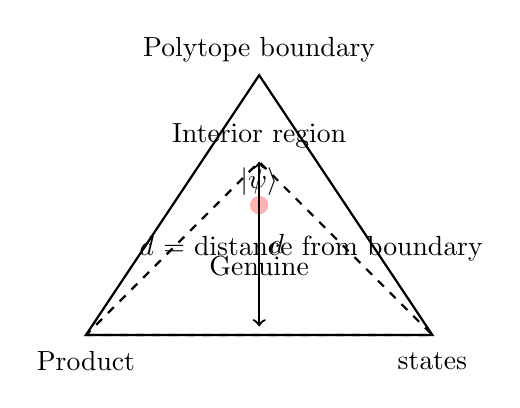
\begin{tikzpicture}[scale=1.1]
		\draw[thick] (0,0) -- (4,0) -- (2,3) -- cycle;
		\draw[dashed, thick] (0,0) -- (4,0) -- (2,2) -- cycle;

		\fill[red!30] (2,1.5) circle (3pt);
		\node[above] at (2,1.5) {$|\psi\rangle$};

		\node at (2,3.3) {Polytope boundary};
		\node at (2,2.3) {Interior region};
		\node at (0,-0.3) {Product};
		\node at (4,-0.3) {states};
		\node at (2,0.8) {Genuine};

		\draw[<->, thick] (2,0.1) -- (2,2) node[midway, right] {$d$};
		\node at (2.6,1) {$d$ = distance from boundary};

	\end{tikzpicture}
	\caption{Entanglement polytope showing the position of a state $|\psi\rangle$ within the polytope. The distance from the boundary indicates the amount of genuine multipartite entanglement. Extreme points (vertices) correspond to product states, while the interior contains genuinely multipartite entangled states. Entanglement vector position: A state's position within the polytope indicates its entanglement. The distance $d$ from the boundary measures how "genuinely" entangled the state is. States near the boundary have less genuine multipartite entanglement.}
	\label{fig:entanglement-polytope-position}
\end{figure}
